\begin{frame}
	\setbeamercolor{block body}{bg = yellow}
	\begin{block}{}
		\begin{center}
			{\large\textbf{Corso di base JAVA}}\\
			\itshape{Mauro Donadeo}\\
			mail: mauro.donadeo@gmail.com
		\end{center}
	\end{block}
	\setbeamercolor{block body}{bg = white}
	\begin{block}{}	
		\begin{center}
			\large{Le decisioni}\\
			
\includegraphics[width = 30mm]{images/java-logo.jpg}
		\end{center}
	\end{block}	
\end{frame}

\section*{L'enunciato if}
\begin{frame}
\frametitle{Enunciato if}
\begin{block}{}
Il programma \textbf{BankAccount} consente di prelevare tutto il denaro che si vuole
\begin{itemize}
\item il saldo \texttt{balance} può diventare \textbf{\textCl{negativo}}
\begin{itemize}
\item \textbf{balance = balance - amount;}
\end{itemize}
\item \`E una situazione assai poco realistica
\item Quindi il programma deve \textbf{\alert{controllare}} il saldo ed agire di conseguenza. \textit{Consentire il prelievo o no.}
\end{itemize}
\end{block}
\end{frame}

\subsection*{A cosa serve}
\begin{frame}
\begin{columns}
\begin{column}{.5\textwidth}
\begin{block}{}
\textbf{\alert{if (amount $<=$ balance)}}\\
\hfill{\textbf{\textCl{balance = balance - amount;}}}
\end{block}
\begin{block}{}
\begin{itemize}
\item L'enunciato if si usa per realizzare una decisione ed è diviso in due parti
\begin{itemize}
\item una \alert{verifica}
\item un \alert{corpo}
\end{itemize}
\item Il corpo viene eseguito \textbf{\textCl{se e solo se} la verifica ha successo}
\end{itemize}
\end{block}
\end{column}
\begin{column}{.5\textwidth}
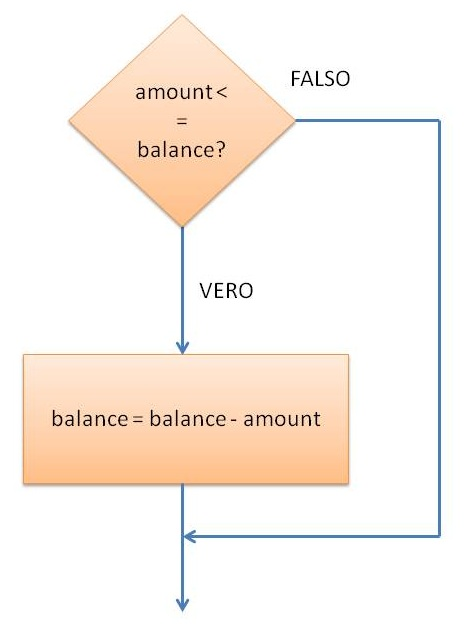
\includegraphics[width = \textwidth]{images/costruttoIf.jpg}
\end{column}
\end{columns}
\end{frame}

\begin{frame}
\frametitle{Tipi di enunciato in Java}
\begin{block}{}
\begin{itemize}
\item Enunciato semplice
\begin{itemize}
\item \textbf{balance = balance - amount;}
\end{itemize}
\item Enunciato composto
\begin{itemize}
\item \textbf{if(x $>=$ 0) x=0;}
\end{itemize}
\item blocco di enunciati
\begin{itemize}
\item \textbf{$\left \{ \mbox{\textbf{\alert{zero o più enunciati di qualsiasi tipo}}} \right \}$}
\end{itemize}
\end{itemize}
\end{block}
\end{frame}
\subsection*{If\ldots then\ldots else\ldots}
\begin{frame}
\begin{block}{}
Proviamo ad emettere un messaggio d'errore in caso di prelievo non consentito:\\
\textbf{if(\alert{amount $<=$ balance})}\\
\hspace{0.7cm}\textbf{balance = balance - amount;}\\
\textbf{if(\alert{amount $>$ balance})} \\
\hspace{0.7cm}\textbf{System.out.println(``Conto scoperto'');} 
\end{block}
\begin{block}{Problema}
Se si modifica la prima verifica, bisogna ricordarsi di modificare anche la seconda.
\end{block}
\begin{block}{Problema}
Se il corpo del primo \texttt{if} viene eseguito, la verifica del secondo \texttt{if} usa il nuovo valore di \texttt{balance},
introducendo \textbf{\textCl{errore logico}}
\begin{itemize}
\item quando si preleva più della metà del saldo disponibile
\end{itemize}
\end{block}
\end{frame}

\begin{frame}
\frametitle{La clausola else}
\begin{block}{}
Per realizzare un'alternativa, si utilizza la clausola \textbf{\textCl{else}} dell'enunciato \texttt{if}\\
\textbf{if(amount $<=$ balance)}\\
\hspace{0.7cm} \textbf{\textCl{balance = balance - amount;}}\\
\textbf{\alert{else}}\\
\hspace{0.7cm}\textbf{\textCl{System.out.println(``Conto aperto'');}}\\
\end{block}
\begin{block}{}
Vantaggio: ora c'è una sola verifica
\begin{itemize}
\item se la verifica ha successo, viene eseguito il primo corpo dell'enunciato \texttt{if/else}
\item altrimenti, viene eseguito il secondo dopo;
\end{itemize}
\end{block}
\end{frame}

\begin{frame}[fragile]
\begin{lstlisting}
if (amount <= balance)
    balance = balance - amount;
else{
    System.out.println("Conto scoperto");
    balance = balance - OVERDRAFT_PENALTY;
}
\end{lstlisting}
\begin{center}
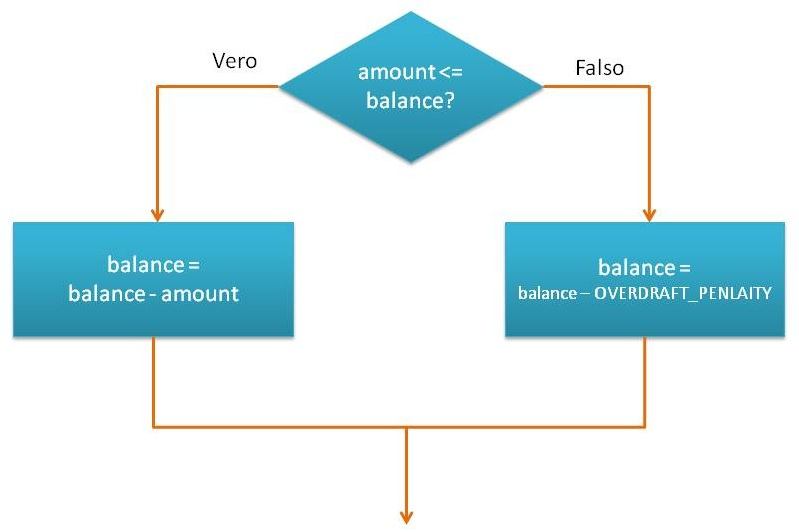
\includegraphics[scale=0.35]{images/costruttoIfElse.jpg}
\end{center}
\end{frame}

\section*{Confronti}
\subsection*{Confronto valori numerici}

\begin{frame}
\begin{block}{}
\begin{huge}
\begin{center}
\textCl{Confrontare valori}
\end{center}
\end{huge}
\end{block}
\end{frame}

\begin{frame}
\begin{block}{}
Le condizioni dell'enunciato if sono molto spesso dei confronti tra due valori\\
\textbf{if(\alert{x $>=$ 0})}\\
Gli operatori di confronto si chiamano operatori relazionali
\end{block}
\begin{block}{}
\centering
\begin{tabular}{|l|l|}
\hline
\textCl{$>$} & Maggiore \\
\hline
\textCl{$>=$} & Maggiore o uguale\\
\hline
\textCl{$<$} & Minore \\
\hline
\textCl{$<=$} & Minore o uguale\\
\hline
\textCl{$==$} & Uguale \\
\hline
\textCl{$!=$} & Diverso\\
\hline
\end{tabular}
\end{block}
\textbf{\alert{Attenzione:}} negli gli operatori da due caratteri \textbf{non} vanno inseriti spazi intermedi 
\end{frame}

\begin{frame}[fragile]
\frametitle{Operatori relazionali}
\begin{block}{}
Fare \textbf{\alert{molta}} attenzione nella differenza tra l'operatore relazionale $==$ e l'operatore assegnazione $=$
\end{block}
\begin{lstlisting}
a = 5; //assegno ad a il valore 5

if(a == 5) //esegue enunciato
   //enunciato
\end{lstlisting}
\end{frame}

\subsection*{Confrontare numeri in virgola mobile}
\begin{frame}
\frametitle{Confrontare numeri in virgola mobile}
\begin{block}{}
I numeri in virgola mobile hanno una precisione limitata ed i calcoli possono introdurre errori di \textCl{arrotondamento} e 
\textCl{troncamento}
\end{block}
\begin{block}{}
Tali errori sono inevitabili e bisogna fare molta attenzione nella formulazione di verifiche che coinvolgono numeri con in 
virgola mobile.
\end{block}
\end{frame}

\begin{frame}
\begin{block}{}
Affinché gli errori di arrotondamento non influenzino la logica del programma, i confronti tra numeri in virgola mobile devono avere
una \textCl{tolleranza}
\end{block}
\begin{block}{}
\begin{itemize}
\item Verifica di uguaglianza tra x ed y (di tipo double): 
\textbf{$$ |x-y| < \epsilon \mbox{ con }\epsilon \mbox{ = 1E-14} $$}
\item Scelta migliore se x,y sono molto grandi o molto piccoli
\textbf{$$|x-y| < \epsilon*max(|x|,|y|) \mbox{ con  }\epsilon \mbox{= 1E-14}$$}
\end{itemize}
\end{block}
\end{frame}

\begin{frame}
\frametitle{Esercizio}
\begin{block}{}
Calcolare la radice quadrata di 2 e confrontare il risultato con 2. Se il risultato è uguale a 2 Stampare ``ok!'' altrimenti ``Errore''
\end{block}
\end{frame}

\subsection*{Confrontare le stringhe}
\begin{frame}
\begin{block}{}
\begin{itemize}
\item Per confrontare stringhe si usa il metodo \textbf{\textCl{equals}}\\
\hspace{0.7cm}\textbf{if(s1.\textbf{\alert{equals(s2)}})}
\item Per confrontare stringhe ignorando la differenza tra maiuscole e minuscole si usa \textbf{\textCl{equalsIgnorecase}}\\
\hspace{0.7cm}\textbf{if(s1.\textbf{\alert{equalsIgnorecase(s2)}})}
\item Non usare \textbf{\alert{mai}} l'operatore di ugualianza per confrontare stringhe. \textbf{\textCl{Usare sempre equals}}
\begin{itemize}
\item Attenzione perché la Virtual Machine \textbf{\alert{NON}} segnalerà alcun errore di sintassi
\end{itemize}
\end{itemize}
\end{block}
\end{frame}

\begin{frame}[fragile]
\frametitle{Confronto di stringhe}
\begin{block}{}
Confrontando con l'operatore di uguaglianza due riferimenti a stringhe si verifica se i riferimenti puntano allo stesso oggetto stringa
\end{block}
\begin{lstlisting}
String s1 = "Stringa";
String s2 = s1;
String s3 = "String";
s3 = s3 + "a"; // s3 contiene "Stringa"
\end{lstlisting}
\pause
\begin{block}{}
\begin{itemize}
\item Il confronto \textbf{s1 $==$ s2 è \textCl{vero}}, perché puntano allo stesso oggetto stringa
\item Il confronto \textbf{s1 $==$ s3 è \textCl{falso}}, perché puntano ad oggetti diversi, anche se tali oggetti hanno lo stesso contenuto 
(sono ``identici'')
\end{itemize}
\end{block}
\end{frame}
\begin{frame}
\frametitle{Ordinamento lessicografico}
\begin{block}{}
\begin{itemize}
\item Se due stringhe sono diverse, è possibile conoscere la relazione che intercorre tra loro secondo \textbf{\textCl{l'ordinamento 
lessicografico}}, simile al comune ordinamento alfabetico.
\item Il confronto lessicografico tra stringhe si esegue con il metodo \textbf{compareTo}\\
\hspace{0.7cm}\textbf{if(s1.\alert{compareTo}(s2) $<$ 0)}
\item Il metodo compareTo restituisce in valore \texttt{int}
\begin{itemize}
\item \textbf{negativo} se s1 precede s2 nell'ordinamento;
\item \textbf{positivo} se s1 segue s2 nell'ordinamento;
\item \textbf{zero} se s1 e s2 sono identiche.
\end{itemize}
\end{itemize}
\end{block}
\end{frame}

\begin{frame}
\frametitle{Esercizio}
\begin{block}{}
Scrivere un programma che chiede all'utente di inserire tre stringhe (una per riga) visualizza le stringhe in ordine lessicografico 
crescente (una per riga)
\end{block}
\end{frame}

\subsection*{Confronto di oggetti}
\begin{frame}
\frametitle{Confronto di oggetti}
\begin{block}{}
\begin{itemize}
\item Come per le stringhe, l'operatore $==$ tra due variabili oggetto verifica se i due riferimenti puntano allo stesso oggetto, 
e \alert{non} verifica l'uguaglianza tra oggetti
\item Il metodo \textbf{equals} può essere applicato a qualsiasi oggetto, perché è definito nella classe \textbf{Object}, da cui derivano 
tutte le classi
\item \`E compito di ciascuna classe \textbf{ridefinire} il metodo \textbf{equals}, come per la classe \textbf{String}
\begin{itemize}
\item altrimenti il metodo \textbf{equals} di \textbf{Object} usa semplicemente l'operatore di uguaglianza.
\end{itemize}
\item il metodo \textbf{equals} di ciascuna classe deve effettuare il \textbf{\textCl{confronto delle caratteristiche}} (variabili 
di esemplare) degli oggetti di tale classe
\end{itemize}
\end{block}
\end{frame}

\section*{Alternative multiple}
\subsection*{Sequenza di confronti}
\begin{frame}[fragile]
\frametitle{Sequenza di confronti}
\begin{block}{}
Se si hanno più di due alternative, si usa \textbf{\textCl{sequenza di confronti}}
\end{block}
\begin{lstlisting}
if (voto >= 8)
    System.out.println("Compito Eccellente");
else if (voto >= 6)
    System.out.println("Compito sufficiente");
else if (voto >= 4)
    System.out.println("Compito quasi sufficiente");
else if (voto >= 2)
    System.out.println("Compito insufficiente");
else if (voto >= 0)
    System.out.println("Compito totalmente insufficiente");
else
    System.out.println("Numeri negativi non validi");
\end{lstlisting}
\end{frame}

\begin{frame}[fragile]
\begin{lstlisting}
if (voto >= 0)
    System.out.println("Totalmente insufficiente");
else if (voto >= 2)
    System.out.println("Compito insufficiente");
else if (voto >= 4)
    System.out.println("Compito quasi insufficiente");
else if (voto >= 6)
    System.out.println("Compito sufficiente");
else
    System.out.println("Compito eccellente");
\end{lstlisting}
\pause
\begin{block}{}
\begin{itemize}
\item Il codice seguente non funziona, perché stampa sempre \textbf{Totalmente insufficiente} per qualsiasi valore di voto. 
\item Se si fanno confronti di tipo \textbf{maggiore di} si devono scrivere prima i valori più alti e viceversa.
\end{itemize}
\end{block}
\end{frame}

\begin{frame}[fragile]
\begin{lstlisting}
if (voto >= 8)
    System.out.println("Compito Eccellente");
if (voto >= 6)
    System.out.println("Compito sufficiente");
if (voto >= 4)
    System.out.println("Compito quasi sufficiente");
if (voto >= 2)
    System.out.println("Compito insufficiente");
if (voto >= 0)
    System.out.println("Compito totalmente insufficiente");
\end{lstlisting}
\pause
\begin{block}{}
Se non si rendono \textbf{\textCl{mutuamente esclusive}} le alternative, usando le clausole \textbf{else}, non funziona
\begin{itemize}
\item se voto vale ``3'', stampa \textbf{\alert{sia}} ``Compito insufficiente'' che \textbf{\alert{sia}} ``Compito totalmente 
insufficiente''
\end{itemize}
\end{block}
\end{frame}

\subsection*{Diramazioni annidate}
\begin{frame}
\frametitle{Diramazioni annidate}
\begin{table}[t]
\begin{tabular}{c c c c}
\hline
\multicolumn{2}{c}{Se il vostro stato civile} & \multicolumn{2}{c}{Se il vostro stato civile}\\
\multicolumn{2}{c}{è non coniugato} & \multicolumn{2}{c}{coniugato}\\
\hline
\textbf{Scaglione fiscale} & \textbf{Aliquota} & \textbf{Scaglione fiscale} & \textbf{Aliquota}\\
\hline
\$0 \ldots \$21 450 & 15\% & \$0 \ldots \$35 800 & 15\%\\
\hline
\$21 450 fino a \$51 900 & 28\% & \$38 500 \ldots 86 500 & 28\%\\
\hline
Superiore a \$51 900 & 31\% & Superiore \$86 500 & 31\%\\
\hline
\end{tabular}
\end{table}
\begin{block}{}
Ci sono \textbf{\alert{due livelli}} nel processo decisionale
\begin{itemize}
\item \textbf{\textCl{Prima}}, dobbiamo scegliere lo stato civile
\item \textbf{\textCl{Poi}}, per ciascuno stato civile, dobbiamo scegliere lo scaglione di reddito.
\end{itemize}
\end{block}
\end{frame}

\begin{frame}
\frametitle{Esercitazione}
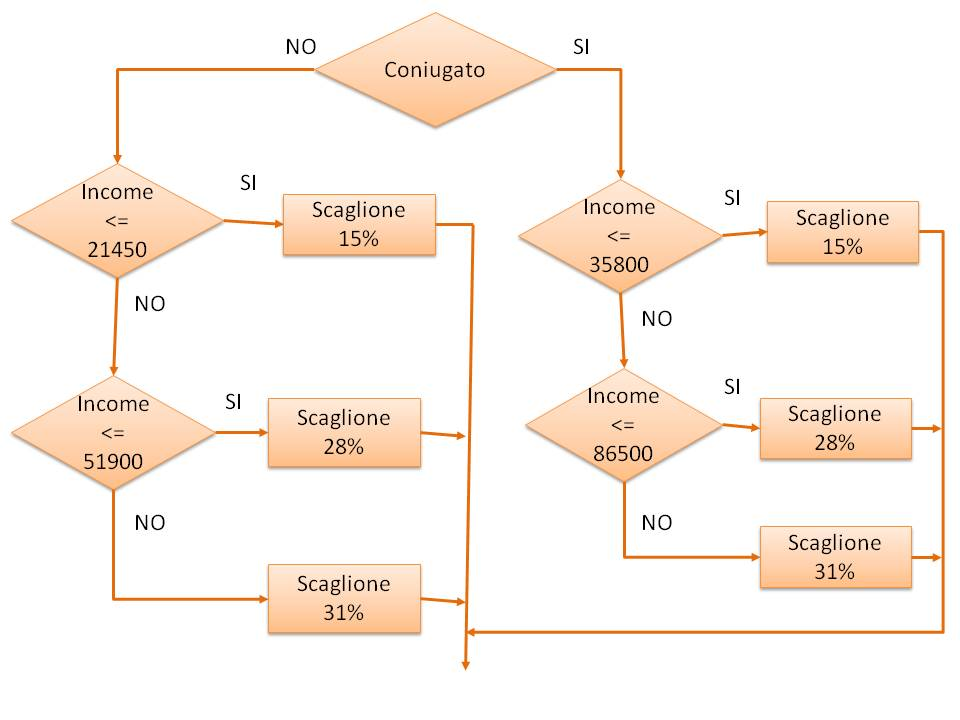
\includegraphics[scale=0.45]{images/eserc1.jpg}
\end{frame}

\subsection*{Else sospeso}
\begin{frame}[fragile]
\begin{block}{}
Nell'esempio precedente abbiamo notato che, se ben indentato il codice, la clausola else si riferisce al primo enunciato \textbf{if}
La regola sintattica è che \textbf{una clausula else appartiene sempre all'enunciato if più vicino}
\end{block}
\begin{lstlisting}
double cost = 5; // prezzo per USA
if (country.equals("USA"))
    if (state.equals("HI"))
        cost = 10; // Hawaii piu' costoso
else
   cost = 20; // estero ancora piu' costoso
\end{lstlisting}
\end{frame}

\begin{frame}[fragile]
\begin{block}{}
L'esempio precedente svolge la funzione seguente con la giusta indentazione
\end{block}
\begin{lstlisting}
double cost = 5; // prezzo per estero
if (country.equals("USA"))
    if (state.equals("HI"))
        cost = 10; // Hawaii piu' costoso
    else
        cost = 20; // USA ancora piu' costoso
\end{lstlisting}
\begin{block}{}
Il risultato è che gli stati esteri ottengono il prezzo più basso, e gli USA continentali il più alto! Il \textbf{contrario} di ciò che 
si voleva\ldots
\end{block}
\end{frame}

\begin{frame}[fragile]
Per ottenere il risultato voluto, bisogna ``nascondere'' il secondo enunciato if all'interno di un blocco di enunciati, inserendo una 
coppia di parentesi graffe.
\begin{itemize}
\item per evitare problemi con \textbf{else} sospeso, è meglio \textbf{\alert{racchiudere sempre}} il corpo di un enunciato if tra 
parentesi graffe, anche quando sono inutili.
\end{itemize}
\begin{lstlisting}
double cost = 5; // prezzo per USA
if (country.equals("USA")){ 
    if (state.equals("HI"))
    cost = 10; // Hawaii piu' costoso
}else
    cost = 20; // estero ancora piu' costoso
\end{lstlisting}
\end{frame}

\section*{Espressioni booleane}
\begin{frame}
\begin{huge}
\begin{center}
\textbf{\textCl{Espressioni booleane}}
\end{center}
\end{huge}
\end{frame}

\subsection*{Il tipo di dati booleano}
\begin{frame}
\begin{block}{}
Ogni espressione in Java ha un \textbf{valore}
\begin{itemize}
\item \textbf{$x + 10 $} espressione aritmetica, valore \textCl{numerico};
\item \textbf{$x < 10 $} espressione relazionale, valore \textCl{booleano};
\end{itemize}
Una espressione relazionale può avere solo due valori \textbf{\alert{true}} o \textbf{\alert{false}}
\end{block}
\end{frame}

\begin{frame}
\begin{block}{}
\begin{itemize}
\item Il tipo di dati \textbf{boolean}, come tutti gli altri tipi di dati, consente la definizione di variabili
\item A volte è comodo utilizzare \textbf{\textCl{variabili booleane}} per memorizzare valori di passaggi intermedi in cui è opportuno
scomporre verifiche troppo complesse
\item Altre volte l'uso di una variabile booleana rende più leggibile il codice
\end{itemize}
\end{block}
\begin{block}{Metodi predicativi}
Così vengono chiamati i metodi che restituiscono valori di tipo \textbf{booleano}.
\begin{itemize}
\item Solitamente \textbf{\textCl{verificano}} una condizione sullo stato di oggetto
\item Solitamente iniziano con \textbf{is} oppure \textbf{has}
\end{itemize}
Metodi predicativi possono essere usati come condizioni di enunciati \textbf{if}
\end{block}
\end{frame}

\subsection*{Operatori booleani}
\begin{frame}
\frametitle{Gli operatori booleani o logici}
\begin{block}{}
Gli operatori booleani o logici servono a svolgere \textbf{\alert{operazioni su valori booleani}}
\end{block}
\hspace{0.7cm}\textbf{if($x > 10 \mbox{ \&\& } x < 20$)} 
\begin{block}{}
\begin{itemize}
\item L'operatore \textbf{\&\&} (and) combina due o più condizioni in una sola, che risulta vera \textbf{\alert{se e solo se sono tutte 
vere}}.
\item L'operatore \textbf{$\|$} (or) combina due o più condizioni in una sola, se risulta vera \textbf{\alert{se e solo se almeno 
una è vera}}
\item L'operatore \textbf{!} (not) \textbf{\alert{inverte}} il valore di una espressione booleana
\end{itemize}
\end{block}
\end{frame}

\begin{frame}
\begin{block}{}
Più operatori booleani possono essere usati in un'unica espressione
\end{block}
\hspace{0.7cm}\textbf{if(($x > 10 \mbox{ \&\& } x > 20$) $\| \mbox{ } x > 30$)}
\begin{block}{}
La valutazione di un'espressione con operatori booleani viene effettuata con una strategia detta cortocircuito (o 
\textbf{valutazione pigra})
\end{block}
\end{frame}


\begin{frame}
\begin{block}{AND}
\centering
\begin{tabular}{|c|c|c|}
\hline
A & B & A$\&\&$B\\
\hline
true & true & true\\
\hline
true & false & false\\
\hline
false & qualsiasi & false \\
\hline
\end{tabular}
\end{block}

\begin{block}{OR}
\centering
\begin{tabular}{|c|c|c|}
\hline
A & B & A $\|$ B\\
\hline
true & qualsiasi & true\\
\hline
false & true & true\\
\hline
false & false & false \\
\hline
\end{tabular}
\end{block}

\begin{block}{NOT}
\centering
\begin{tabular}{|c|c|}
\hline
A & !A\\
true & false\\
\hline
false & true\\
\hline
\end{tabular}
\end{block}
\end{frame}

\begin{frame}[fragile]
\begin{block}{}
\begin{itemize}
\item In un'espressione booleana con più operatori, la valutazione viene fatta da sinistra a destra, dando la precedenza all'operatore 
\textbf{not}, poi all'operatore \textbf{and}, infine all'operatore \textbf{or}
\item L'ordine di valutazione può comunque essere alterato dalle parentesi tonde
\end{itemize}
\end{block}
\begin{lstlisting}
if (!(x < 0 || x > 10)){
    // esegue se x e' compreso tra 0 e 10,
    // estremi inclusi
}
\end{lstlisting}
\begin{lstlisting}
if (!x < 0 || x > 10)
  // esegue se x e' maggiore o uguale a 0
\end{lstlisting}
\end{frame}

\begin{frame}
\frametitle{ESERCITAZIONE}
\begin{block}{}
Scrivere un programma che segnala all'utente se il numero intero positivo che ha introdotto corrisponde ad un anno bisestile oppure no.
\end{block}
\begin{block}{}
\textbf{Suggerimento}: un anno bisestile è divisibile per 4. Fanno eccezione gli anni divisibili per 100, che non sono bisestili, e gli 
anni divisibili per 400, che invece sono bisestili: tali eccezioni esistono però solo dopo l'adozione del calendario gregoriano, che 
avvenne nel 1582.
\end{block}
\end{frame}

\begin{frame}[fragile]
\begin{block}{}
Si scriva la classe Triangolo, che descrive un triangolo. 
\end{block}
\begin{block}{}
Collaudare la classe Triangolo con la classe di prova TriangoloTester, che legge i dati da standard input
\end{block}
\end{frame}